\documentclass{article}
\usepackage{amsmath}
\usepackage{graphicx}
\usepackage{hyperref}
\usepackage[all]{hypcap} % Make \autoref links jump to TOP of figures, not their captions
\usepackage{float} % Put figures exactly where they are in the code with [H]


\usepackage[letterpaper,margin=1in]{geometry}

\title{{\sffamily PageRank with Eigenvectors}
{\sc cla365 technical report }}

\author{Nathaniel Reimer \and Preston Locke}
\date{April 30, 2022}

\begin{document}
\maketitle

\begin{abstract} 
\noindent
In this report we examine the PageRank algorithm by showing that the Google Matrix is stochastic. We then present R code that implements the PageRank algorithm and demonstrate it on a simple network. As an extension, we explore some permutations on this network as well as the implications of changing the random jump probability ($q$)
\end{abstract}


\section{Implementing PageRank}

\subsection{Proving the Google Matrix is Stochastic}


Proving the Google matrix $G$ is stochastic requires showing that $G$ is nonnegative
and that each of its columns sum to $1$. We'll start by proving that the matrix is
nonnegative. Note that for each entry in $G$, we have the following:

$$
G_{ij} = q/n + A_{ji} (1 - q) / n_j
$$

We already know the following facts about the variables in the expression above:

\begin{enumerate}
    \item $0 \leq q \leq 1$
    \item $n > 0$
    \item $A_{ji} \in \{0,1\}$
    \item $n_j = \sum_{i=1}^n A_{ji}$
\end{enumerate}

From facts 1, 2, and 3, we also know that $q/n$, $A_{ji}$, and $(1 - q)$ are all
nonnegative numbers. And then, by facts 3 and 4, $n_j$ must also be nonnegative. Therefore,
we can say that the entire expression is nonnegative, and thus, each entry in $G$ is
nonnegative by definition.

Next, we show that each column in $G$ sums to $1$, or in other words, that for each
$j \in \{ 1, 2, ..., n\}$ we show that:

$$
\sum_{i=1}^n q/n + A_{ji} (1 - q) / n_j = 1
$$

The first term in the summation can be pulled out because it's easy to see that $q/n$
added $n$ times will just equal $q$. We can also pull out the expression
$((1 - q) / n_j)$ from the summation, because everything in it is a constant with
respect to $i$. Doing these two things gives us the below:

$$
q +  ((1 - q) / n_j) \sum_{i=1}^n A_{ji}
$$

Now, using fact 4 from the first part of our proof, we can simplify $\sum_{i=1}^n A_{ji}$
to $n_j$ and finish simplifying:

$$
q +  ((1 - q) / n_j) n_j
$$
$$
q + (1 - q)
$$
$$
1
$$

With that, we have successfully shown that $G$ is a nonnegative matrix whose columns sum
to $1$, so we have proven that $G$ is stochastic.

\subsection{Calculating the Google Matrix and Page Ranks}

To calculate page ranks for a given network of pages, we can use the fact that $G$ is
stochastic and find its dominant eigenvector, which will give us the rankings. If we
scale that eigenvector so that its entries sum to $1$, we'll have our answer. To do
this, we've written two R functions, GoogleMatrix and PageRankVector,
which take in an $n \times n$ adjacency matrix adj and output, respectively,
the $n \times n$ Google matrix of the network and a vector of page ranks given the value
of q (which defaults to $0.15$).

\begin{verbatim}
GoogleMatrix = function(adj, q=0.15) {
  n = dim(adj)[1]
  G = matrix(nrow=n, ncol=n)
  
  for (j in 1:n) {
    # Get the sum of row j
    n.j = sum(adj[j,])
    
    for (i in 1:n) {
      # Calculate the ijth entry of G
      G[i,j] = q/n + adj[j,i] * (1 - q) / n.j
    }
  }
  
  return(G)
}

PageRankVector = function(adj, q=0.15) {
  G = GoogleMatrix(adj, q=q)
  
  # Find the dominant eigenvector of G
  p = eigen(G)$vectors[,1]
  
  # Return the normalized version (inf. norm)
  return(p / sum(p))
}
\end{verbatim}

\begin{figure}[H]
$$
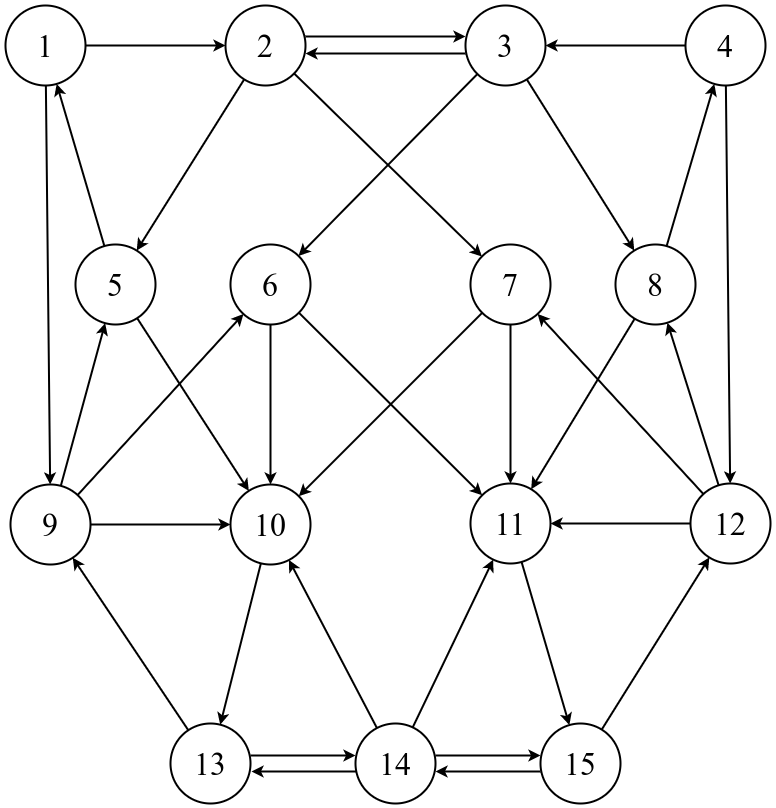
\includegraphics[width=2in]{images/network-1.png} 
$$
\vspace{-0.25in}
\caption{Network of 15 pages, taken from page 550 of the textbook.}
\label{fig:network1}
\end{figure}


We can test these functions on the network in \autoref{fig:network1} that is taken from
the textbook. The result of running GoogleMatrix is shown in \autoref{appendix:googlematrix}, but the result of running PageRankVector is
shown below:

\begin{small}
\begin{verbatim}
> A = rbind(
+     c(0,1,0,0,0,0,0,0,1,0,0,0,0,0,0),
+     c(0,0,1,0,1,0,1,0,0,0,0,0,0,0,0),
+     c(0,1,0,0,0,1,0,1,0,0,0,0,0,0,0),
+     c(0,0,1,0,0,0,0,0,0,0,0,1,0,0,0),
+     c(1,0,0,0,0,0,0,0,0,1,0,0,0,0,0),
+     c(0,0,0,0,0,0,0,0,0,1,1,0,0,0,0),
+     c(0,0,0,0,0,0,0,0,0,1,1,0,0,0,0),
+     c(0,0,0,1,0,0,0,0,0,0,1,0,0,0,0),
+     c(0,0,0,0,1,1,0,0,0,1,0,0,0,0,0),
+     c(0,0,0,0,0,0,0,0,0,0,0,0,1,0,0),
+     c(0,0,0,0,0,0,0,0,0,0,0,0,0,0,1),
+     c(0,0,0,0,0,0,1,1,0,0,1,0,0,0,0),
+     c(0,0,0,0,0,0,0,0,1,0,0,0,0,1,0),
+     c(0,0,0,0,0,0,0,0,0,1,1,0,1,0,1),
+     c(0,0,0,0,0,0,0,0,0,0,0,1,0,1,0)
+ )
> PageRankVector(A)
 [1] 0.027 0.030 0.030 0.027 0.040 0.040 0.040 0.040 0.075 0.106 0.106 0.075 0.125 0.116 0.125
\end{verbatim}
\end{small}

Higher numbers in the PageRank vector correspond to higher rankings. So, using the PageRank
method with $q$=.15 makes 13 and 15 the highest ranked websites and 1 and 4 the lowest ranked. 

\section{Further Exploration}

\subsection{Other Values of q}
The jump probability, $q$, is the probability that a web-surfer chooses any random website rather than clicking one of the links on their current website. We can illustrate this using the equation for the entries to the Google matrix $G$. 
\[G_{ij}=\frac{q}{n}+A_{ij}(1-q)/n_j\]
If \(q=1\) then \(G_{ij}=\frac{q}{n}\) since the other term is multiplied by 0. As we expect, the probability of ending up at any particular website is just $1/n$ where $n$ is the number of websites: after visiting a website a web-surfer simply chooses another website at random from the list. We use the image() function in R to visualize the page rank vector for different values of $q$. In \autoref{fig:pagerank1}, higher values in the PageRank vector are in yellow and lower values are in dark blue. 

\begin{figure}[H]
$$
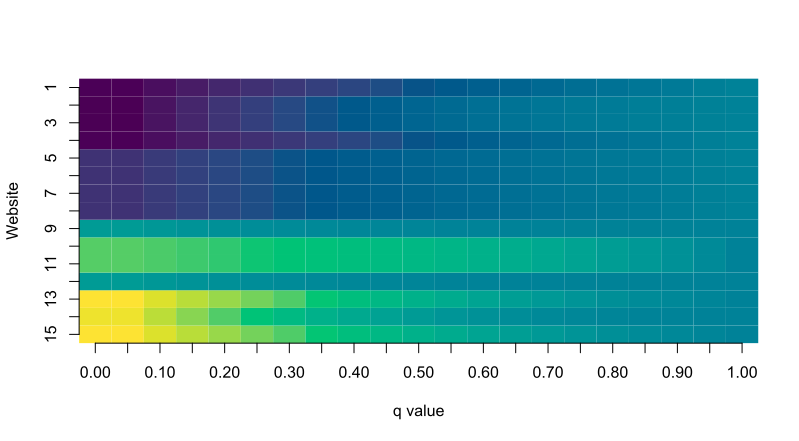
\includegraphics[width=5in]{images/pagerank-Aq-v2.png} 
$$
\vspace{-0.4in}
\caption{Heatmap of PageRank vectors at different q values.}
\label{fig:pagerank1}
\end{figure}


The result we obtain from \autoref{fig:pagerank1} is precisely what we expect. At a $q$ value of 1 all of the websites' entries in the PageRank vector are exactly equal (they are the same color). Moreover, as we decrease $q$ differences appear and become more pronounced. When $q$ is zero and the probability of ending up at any given website is based solely on the network structure: There are no random jumps. For PageRank, Google used a q value of .15 so that network structure is the primary determining factor but some random jumping occurs. 
This choice has a number of interesting implications for our network. We first observed that while 15, 14, and 13 have similar values when $q$ is zero, when $q$ reaches .15 website 14 has fallen further than 13 and 15. Additionally, 2 and 3 have lower values when $q$ is zero but higher values when $q$ is .15. It would be unrealistic to assume there is no random jumping when someone is surfing the web and not accounting for it leads to an incorrect page rank, especially in the case of 1, 2, 3, and 4. Why, exactly, these changes happen in this network is certainly worthy of further study. It may come about because of the symmetric connections between 2 and 3 and those between 13, 14, and 15.


\subsection{Removing a Node}
 
\begin{figure}[H]
$$
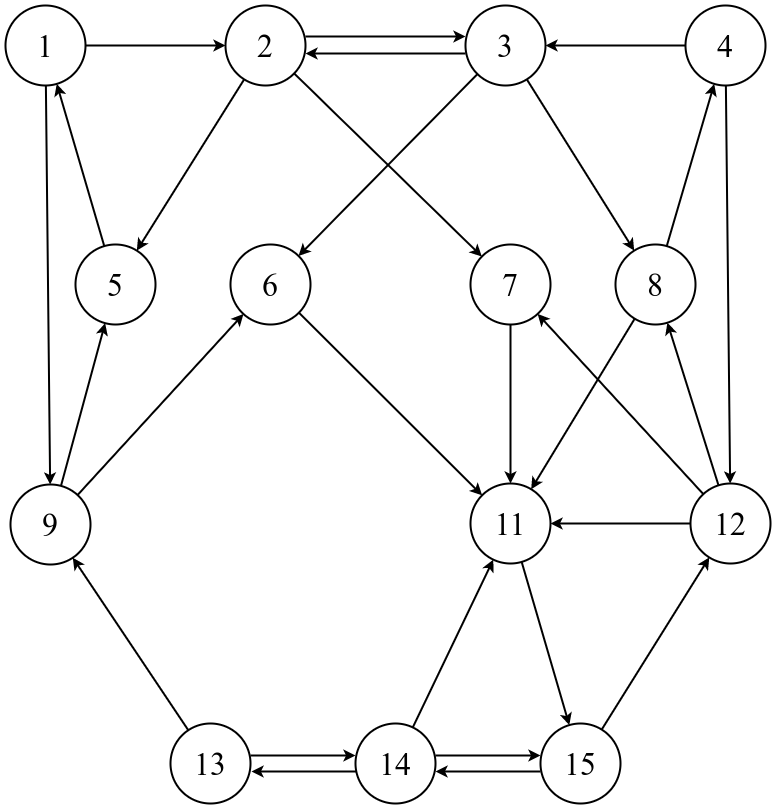
\includegraphics[width=2in]{images/network-3.png} 
$$
\vspace{-0.25in}
\caption{Network with Page 10 removed.}
\label{fig:network3}
\end{figure}

What happens to the ranks of the other pages if we remove a page from the network?
For a start, we can predict that the effect on the other page ranks will be more
pronounced when a page with a higher rank is removed. Being a probability
distribution, the page rank vector needs to add to $1$, and thus the value of the
removed page's rank will need to be redistributed to the other pages somehow, in
order to maintain the sum of $1$. The higher the removed page's rank, the more
value will be redistributed to the other pages.

Exploring this theme of removing highly-ranked pages further, let's look at a concrete
example using the 15-page example from before. This time, we'll remove page 10 to get
the network shown in \autoref{fig:network3}. Below are the page ranks we calculated
for the modified network:

\begin{verbatim}
> PageRankVector(A[c(1:9, 11:15), c(1:9, 11:15)])
 [1] 0.047 0.041 0.036 0.032 0.043 0.041 0.052 0.050 0.048 0.171 0.104 0.041 0.107 0.186
\end{verbatim}

Comparing these rankings to those of the 15-page network, we see that almost all of the
pages rose in rank, except for pages 9, 13, and 14. Note that page 13 was pointed to by
page 10, and page 13 points to pages 9 and 14. It seems that the popularity of page 10
contributed to propping up the rankings of pages 9, 13, and 14, so when it was removed,
those page rankings fell.

It should be noted, however, that in the given network, there is a directed path from
page 10 to every other page in the network, meaning that to some degree, all
pages are pointed to by page 10, implying that page 10's popularity should have had
some effect of propping those pages up, if only small. We believe the reason why the
rankings of the other pages did not fall is a combination of their degree of separation from
page 10 (longer paths yield a smaller influence on ranking) and other factors
(like a change in a page's ratio of in-links to out-links).

\subsection{Rank Strategy}

We then considered a possible strategy for a website to increase its PageRank. Specifically, what happens when websites 2 and 12 favor linking to website 7. We model this by changing the corresponding entries in the adjacency matrix from 1 to 2. In \autoref{fig:network2} we show this change by bolding these two links. We then calculated the PageRank vector $p_2$ for the modified matrix and calculated a ratio of it and the original PageRank vector $p_1$ to obtain a vector $\frac{p_2}{p_1}$. 

\[(p_2/p_1)^T=\]
\begin{small}
\begin{verbatim}
      [,1]  [,2]  [,3]  [,4]  [,5]  [,6] [,7]  [,8] [,9] [,10] [,11] [,12] [,13] [,14] [,15]
[1,] 0.969 0.954 0.878 0.892 0.951 0.986 1.33 0.829 1.02  1.05 0.971  0.97  1.04  1.01 0.981
\end{verbatim}
\end{small}
\begin{figure}[H]
    \centering
    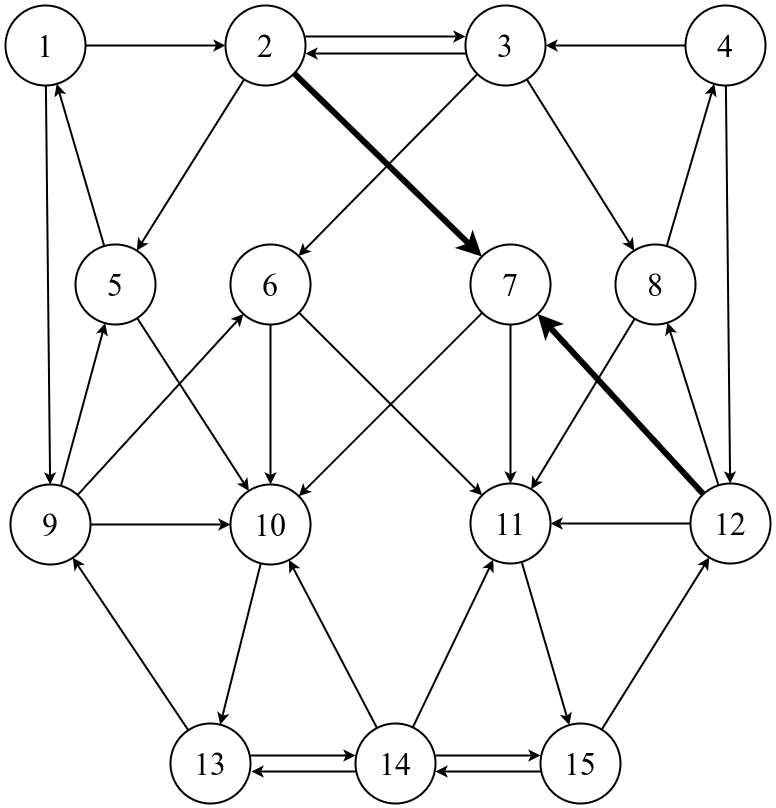
\includegraphics[width=2in]{images/network-2.png} 
    \caption{Modified network with more prominent links to website 7.}
    \label{fig:network2}
\end{figure}


Unsurprisingly, strategy has benefited page 7's value in the PageRank vector. We decided to take a closer look at how the strategy impacted the values of other sites. We immediately noticed that while 11 and 10 are both linked to by page 7, only page 10's value increased. This can be explained by examining the network structure. In the google matrix for the modified network the probability of moving from 12 to 7 is increased, this means that the probability of moving from 12 to 11 or 4 is decreased. So even though 11 may benefit from being linked to by 7 this is out weighed by the negative effect of being deprioritized by 12. 10 does not face this negative effect and thus benefits. 




\newpage
\appendix

\section{Appendix: Unmodified 15-Page Google Matrix}
\label{appendix:googlematrix}

\begin{small}
\begin{verbatim}
> GoogleMatrix(A)
      [,1] [,2] [,3] [,4] [,5] [,6] [,7] [,8] [,9] [,10] [,11] [,12] [,13] [,14] [,15]
 [1,] 0.01 0.01 0.01 0.01 0.43 0.01 0.01 0.01 0.01  0.01  0.01  0.01  0.01  0.01  0.01
 [2,] 0.43 0.01 0.29 0.01 0.01 0.01 0.01 0.01 0.01  0.01  0.01  0.01  0.01  0.01  0.01
 [3,] 0.01 0.29 0.01 0.43 0.01 0.01 0.01 0.01 0.01  0.01  0.01  0.01  0.01  0.01  0.01
 [4,] 0.01 0.01 0.01 0.01 0.01 0.01 0.01 0.43 0.01  0.01  0.01  0.01  0.01  0.01  0.01
 [5,] 0.01 0.29 0.01 0.01 0.01 0.01 0.01 0.01 0.29  0.01  0.01  0.01  0.01  0.01  0.01
 [6,] 0.01 0.01 0.29 0.01 0.01 0.01 0.01 0.01 0.29  0.01  0.01  0.01  0.01  0.01  0.01
 [7,] 0.01 0.29 0.01 0.01 0.01 0.01 0.01 0.01 0.01  0.01  0.01  0.29  0.01  0.01  0.01
 [8,] 0.01 0.01 0.29 0.01 0.01 0.01 0.01 0.01 0.01  0.01  0.01  0.29  0.01  0.01  0.01
 [9,] 0.43 0.01 0.01 0.01 0.01 0.01 0.01 0.01 0.01  0.01  0.01  0.01  0.43  0.01  0.01
[10,] 0.01 0.01 0.01 0.01 0.43 0.43 0.43 0.01 0.29  0.01  0.01  0.01  0.01  0.22  0.01
[11,] 0.01 0.01 0.01 0.01 0.01 0.43 0.43 0.43 0.01  0.01  0.01  0.29  0.01  0.22  0.01
[12,] 0.01 0.01 0.01 0.43 0.01 0.01 0.01 0.01 0.01  0.01  0.01  0.01  0.01  0.01  0.43
[13,] 0.01 0.01 0.01 0.01 0.01 0.01 0.01 0.01 0.01  0.86  0.01  0.01  0.01  0.22  0.01
[14,] 0.01 0.01 0.01 0.01 0.01 0.01 0.01 0.01 0.01  0.01  0.01  0.01  0.43  0.01  0.43
[15,] 0.01 0.01 0.01 0.01 0.01 0.01 0.01 0.01 0.01  0.01  0.86  0.01  0.01  0.22  0.01
\end{verbatim}
\end{small}

\end{document}
